% Ver el archivo config.tex ya que contiene templates de código útil y diferentes operadores matemáticos.
\input{config.tex}
% Especificación del encabezado y pie de página.
\fancyhf{}
\lhead{\small TPx [2C2020]}
\chead{}
\rhead{\small [xx.xx] Asignatura}
\rfoot{}
\cfoot{Página {\thepage} de \pageref{LastPage}}
\lfoot{}
%-----------------------------------%
%									%
%		Comienzo del documento		%
%									%
%-----------------------------------%
\begin{document}
%-----------------------------------%
%									%
%			Caratula				%
%									%
%-----------------------------------%
\pagestyle{fancy}
\begin{titlepage}
	\newcommand{\HRule}{\rule{\linewidth}{0.5mm}} % Defines a new command for horizontal lines, change thickness here
	\center % Centre everything on the page
	
	\thispagestyle{empty}
	\begin{center}
		\includegraphics[scale=0.9]{includes/banner_fiuba.pdf}\\
	\end{center}
	
 	\vspace*{\stretch{1}}
	
	\textsc{\Large \textsc{[xx.xx] ASIGNATURA}}\\[0.3cm]
	\textsc{\Large \textsc{Trabajo Práctico X}}\\[0.3cm]
	\textsc{\large x\textsuperscript{er} Cuatrimestre 2019}\\[0.25cm]
	
	\HRule\\[0.2cm]
	{\large\bfseries TITULO TITULO TITULO TITULO TITULO TITULO TITULO TITULO TITULO TITULO TITULO TITULO TITULO TITULO TITULO TITULO TITULO TITULO}\\[0.2cm]
	\HRule\\[0.2cm]
	
	\begin{tabbing}
		\hspace{2cm}\=\+
		\underline{AUTOR}\hspace{-1cm}\=\+\hspace{1cm}\=\hspace{6cm}\=\\[0.2cm]
		
		Apellido, Nombre.	\>\>- \#100.000\\
		\>\footnotesize{$<$email@fi.uba.ar$>$}\\
		Apellido, Nombre.	\>\>- \#100.000\\
		\>\footnotesize{$<$email@fi.uba.ar$>$}\\
		Apellido, Nombre.	\>\>- \#100.000\\
		\>\footnotesize{$<$email@fi.uba.ar$>$}\\
		Apellido, Nombre.	\>\>- \#100.000\\
		\>\footnotesize{$<$email@fi.uba.ar$>$}\\
		Apellido, Nombre.	\>\>- \#100.000\\
		\>\footnotesize{$<$email@fi.uba.ar$>$}\\
		Apellido, Nombre.	\>\>- \#100.000\\
		\>\footnotesize{$<$email@fi.uba.ar$>$}\\
		
		\<\underline{CÁTEDRA}\\[0.2cm]
		DOCENTE1 \\
		DOCENTE2 \\
		DOCENTE3 \\
		DOCENTE4 \\
		DOCENTE5 \\
		DOCENTE6 \\[0.2cm]
		
		\<\underline{FECHA DE ENTREGA}\>\>\> 01 de enero de 1900
		\\[0.2cm]
		\<\underline{CALIFICACIÓN}\>\>\> 
		\\[0.2cm]
		
	\end{tabbing}
	
	
 	\vspace*{\stretch{1}}
	
	
\end{titlepage}

%-----------------------------------%
%									%
%			Indice					%
%									%
%-----------------------------------%
\clearpage

\tableofcontents							

\clearpage

%-------------------------------%
%								%
%	Seccion: Objetivos			%
%								%
%-------------------------------%
\clearpage
\section{Objetivos}
El presente trabajo tiene los siguientes objetivos:
\begin{itemize}
	\item Modelar .....
	\item Implementar y validar algoritmos ...
	\item Modelar y simular ...
\end{itemize}

%-------------------------------%
%								%
%	Seccion: Resultados			%
%								%
%-------------------------------%
\section{Resultados}

Una ecuación
\begin{IEEEeqnarray}{rCl}
	\IEEEyesnumber
	A &=& \pi
\end{IEEEeqnarray}

Otra ecuación
\begin{IEEEeqnarray}{rCl}
	\IEEEyesnumber \IEEEyessubnumber*
	A &=& B \\
	B &=& C
\end{IEEEeqnarray}

\begin{figure}[!ht]
	\centering
	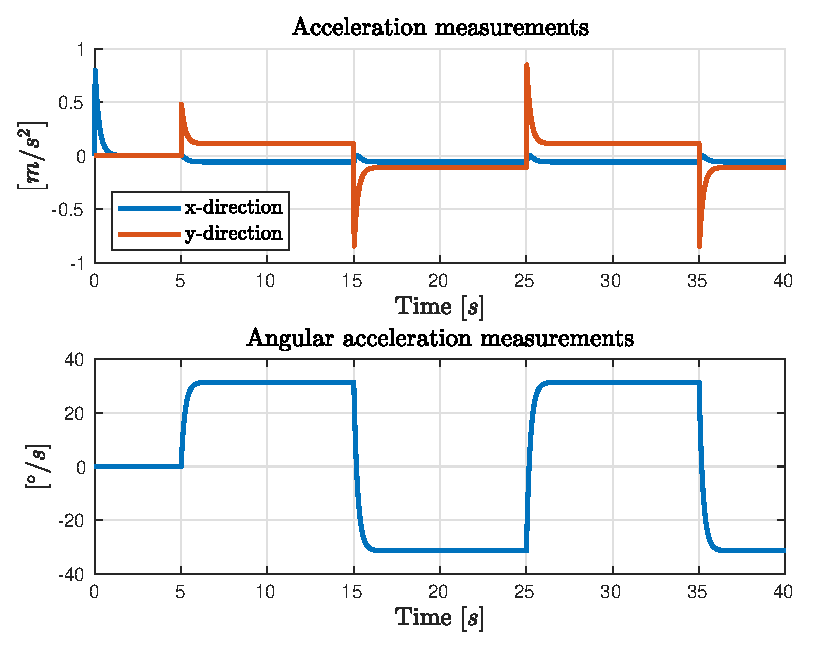
\includegraphics[scale=0.8]{includes/1_measurements_ex1.eps}
	\caption{Mediciones entregadas por los acelerómetros y el giróscopo.} \label{1_measurements_ex1}
\end{figure}

\begin{figure}[h]
	\centering
	\includegraphics[scale=0.7]{includes/4_sistemas_camara.pdf}
	\caption{Relaciones entre sistemas de referencia y ángulo medido por la cámara abordo de un robot.} \label{4_sistemas_camara}
\end{figure}

\begin{figure}[h]
	\centering
	\includegraphics[scale=0.35]{includes/4_sound_sources_diagram.png}
	\caption{Disposición de las fuentes sonoras.} \label{4_sound_sources_diagram}
\end{figure}


La tabla \ref{tabla_ej2} muestra los resultados obtenidos de la aplicación de un algoritmo numérico para determinar el ángulo $\theta$ y su derivada en función del tiempo $t$.

\begin{table}[h!]
	\centering
	\begin{tabular}{|l|l|l|l|l|}
		\hline
		\multicolumn{1}{|c|}{} & \multicolumn{2}{c|}{\textbf{$\theta_k[\SI{}{\radian}]$}} & \multicolumn{2}{c|}{\textbf{$d\theta_k/dt[\SI{}{\radian\per\second}]$}} \\ \hline
		\multicolumn{1}{|c|}{\textbf{$t_k$}} & \multicolumn{1}{c|}{\textbf{RK1}} & \multicolumn{1}{c|}{\textbf{RK4}} & \multicolumn{1}{c|}{\textbf{RK1}} & \multicolumn{1}{c|}{\textbf{RK4}} \\ \hline
		0.00 & 5.236e-01 & 0.0 & 0.000e+00 &  0.0 \\ \hline
		0.02 & 5.236e-01 & 0.0 & -1.027e-01 & 0.0  \\ \hline
		... &  &  &  &  \\ \hline
		19.92 & 1.082e-04 & 0.0 & 3.342e-04 & 0.0 \\ \hline
		19.94 & 1.149e-04 & 0.0 & 3.063e-04 & 0.0 \\ \hline
	\end{tabular}
	\caption{Resultados obtenidos para RK1 utilizando el set de datos $m=1$, $l=1$, $b=1$, $\theta_0=0.523599$, $\frac{d\theta}{dt}_0=0$ utilizando un paso $h = 0.02$.}
	\label{tabla_ej2}
\end{table}

%---------------------------%
%							%
%	Seccion: Conclusiones	%
%							%
%---------------------------%
\section{Conclusiones}

Se simularon y validaron algoritmos de ..., y se cumplió con el objetivo de ...

%---------------------------%
%							%
%	Seccion: Bibliografía	%
%							%
%---------------------------%
\clearpage
\begin{thebibliography}{10}
	\bibitem{latex} 
	\href{https://tobi.oetiker.ch/lshort/lshort-a5.pdf}{The Not So Short
		Introduction to \LaTeX 2} - Tobias Oetiker - Version 6.3, March 26, 2018.
	\bibitem{Zill} 
	\emph{Ecuaciones diferenciales con problemas de valores en la frontera} - Zill, Dennis G. - Cullen, Michael R. - Thompson 6ta ed. - 2007
	
	\bibitem{Apuntes} 
	\emph{Apuntes del curso Análisis numérico 1 - curso Sassano} - Facultad de Ingeniería - Universidad de Buenos Aires - 2020.
	
\end{thebibliography}

\end{document}
